\documentclass[10pt,a4paper]{article}
\usepackage[T1]{fontenc}
\usepackage[utf8]{inputenc}
\usepackage[english]{babel}
\usepackage[a4paper,margin=0.6in,top=0.5in,bottom=0.5in]{geometry}
\usepackage{enumitem}
\usepackage{xcolor}
\usepackage[hidelinks]{hyperref}
\usepackage{titlesec}
\usepackage{microtype}
\usepackage{graphicx}
\usepackage{tgheros}
\renewcommand{\familydefault}{\sfdefault}
\setlength{\parindent}{0pt}
\setlength{\parskip}{0pt}

% Colors
\definecolor{primary}{RGB}{0,70,130}
\definecolor{accent}{RGB}{60,60,60}

% Section formatting
\titleformat{\section}{\color{primary}\normalsize\bfseries}{}{0em}{\MakeUppercase}[\color{primary}\titlerule]
\titlespacing*{\section}{0pt}{6pt}{3pt}

% List style
\setlist[itemize]{leftmargin=12pt,itemsep=1pt,topsep=2pt,parsep=0pt}

% FontAwesome5 with fallback
\IfFileExists{fontawesome5.sty}{\usepackage{fontawesome5}}{%
  \newcommand{\faEnvelope}{@}
  \newcommand{\faPhone}{Tel:}
  \newcommand{\faMapMarker}{Loc:}
  \newcommand{\faGlobe}{Web:}
  \newcommand{\faGithub}{GH:}
  \newcommand{\faLinkedin}{LI:}
}

\begin{document}

% ======================== HEADER ========================
\noindent
\begin{minipage}[c]{0.80\textwidth}
  {\LARGE\bfseries\color{primary} YOSR BEN NAGRA}\\[3pt]
  {\normalsize\color{accent} Full Stack Developer \;\textbar\; React / Node.js / Java}\\[4pt]
  {\footnotesize
    \faEnvelope\ \href{mailto:yosrbennagra@gmail.com}{yosrbennagra@gmail.com} \;\textbar\;
    \faPhone\ +216 53916040 \;\textbar\;
    \faMapMarker\ Tunis, Tunisia\\[2pt]
    \faGlobe\ \href{https://veinpal.com/apps}{veinpal.com} \;\textbar\;
    \faGithub\ \href{https://github.com/YosrBennagra}{YosrBennagra} \;\textbar\;
    \faLinkedin\ \href{https://www.linkedin.com/in/yosr-ben-nagra/}{yosr-ben-nagra}
  }
\end{minipage}%
\hfill
\begin{minipage}[c]{0.16\textwidth}
  \raggedleft
  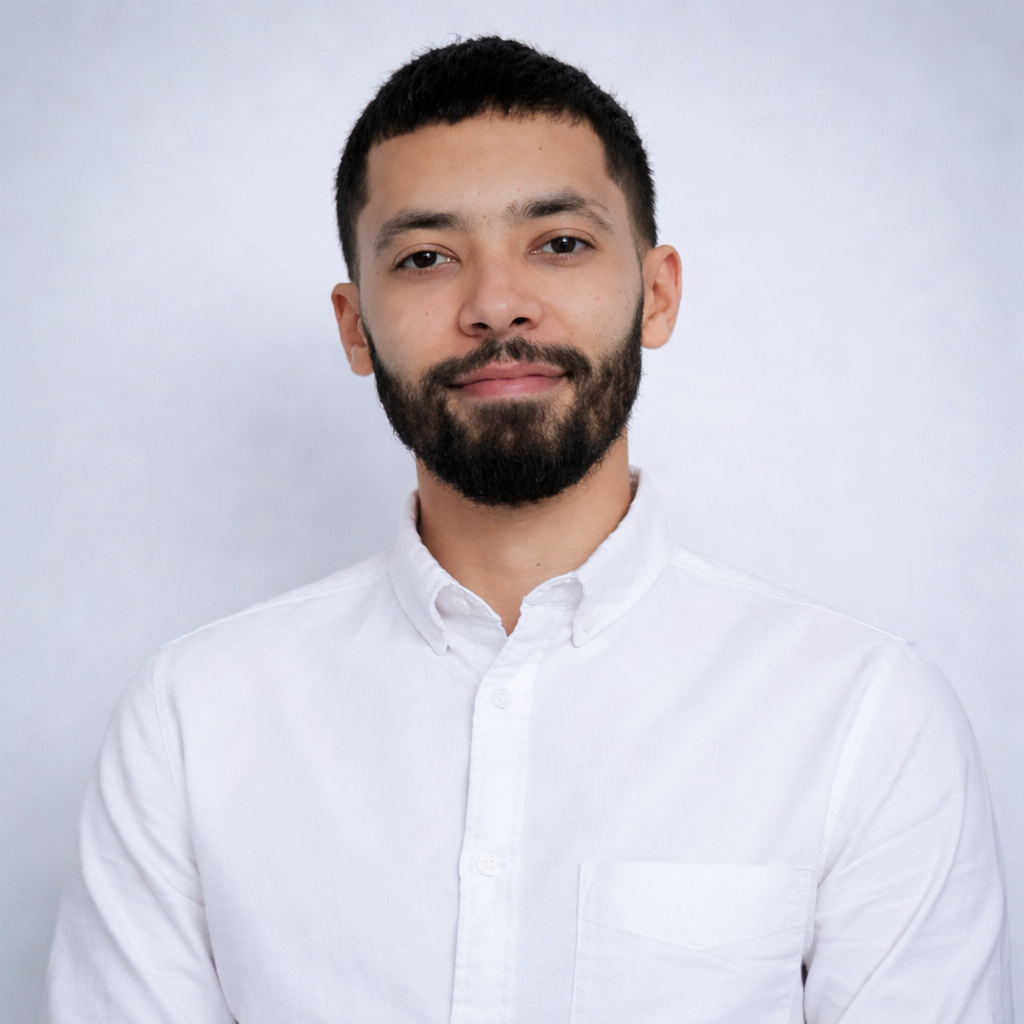
\includegraphics[width=2.2cm,clip]{../../../assets/photo_yosr.png}
\end{minipage}

% ======================== SUMMARY ========================
\section*{Professional Summary}
{\small
Full stack developer and founder of \textbf{Veinpal} (\href{https://veinpal.com/apps}{veinpal.com/apps}), a production platform shipping 5 products to real users. I build end-to-end web applications across the \textbf{React/Next.js}, \textbf{Node.js} (Express, NestJS), \textbf{Java} (Spring Boot), and \textbf{Python} (Flask) ecosystems. Hands-on with \textbf{PostgreSQL}, \textbf{MongoDB}, \textbf{Redis}, and modern DevOps tooling (\textbf{Docker}, \textbf{CI/CD}, monitoring). Strong focus on clean architecture, type safety, automated testing, and delivering measurable value in Agile teams. Fluent English.
}

% ======================== SKILLS ========================
\section*{Technical Skills}
{\small
\textbf{Frontend:} React, TypeScript, JavaScript (ES6+), Next.js, Angular, HTML5, CSS3, Redux Toolkit, Zustand, React Query, React Router\\[2pt]
\textbf{Styling:} Tailwind CSS, shadcn/ui, Material-UI (MUI), Chakra UI, Styled Components, Sass/SCSS, PrimeNG\\[2pt]
\textbf{Backend:} Node.js, Express.js, NestJS, Fastify, Java (8/17/21), Spring Boot, Python, Flask, GraphQL, REST APIs\\[2pt]
\textbf{Real-time:} WebSockets, Socket.io\\[2pt]
\textbf{Databases \& ORM:} PostgreSQL, MongoDB, Redis, Prisma, TypeORM, Mongoose, SQL\\[2pt]
\textbf{Auth:} JWT, Passport.js, NextAuth.js (OAuth)\\[2pt]
\textbf{Testing:} Jest, React Testing Library, Vitest, Cypress, Playwright\\[2pt]
\textbf{DevOps:} Docker, Git, GitHub Actions, Jenkins, Harness, Nginx, Kubernetes (basics), Helm, Vercel, Netlify\\[2pt]
\textbf{Quality \& Monitoring:} SonarQube, Prometheus, Grafana, ESLint, Prettier, Commitlint\\[2pt]
\textbf{Build \& Tooling:} Vite, Webpack, Turborepo, pnpm Workspaces, Zod\\[2pt]
\textbf{Methods:} Agile/Scrum, TDD, Code Review, CI/CD, Monorepo Architecture
}

% ======================== CURRENT POSITIONS ========================
\section*{Current Positions}
{\small
\textbf{Full Stack Developer (Angular/Spring Boot) -- ERP Application} \hfill \textit{Wico \;\textbar\; 2024 -- Present}\\[1pt]
\textit{Tunis, Tunisia}
\begin{itemize}
  \item Develop an \textbf{ERP application} for a construction company end-to-end with \textbf{Angular} and \textbf{Spring Boot} (part-time 2024--2025, full-time since 2026)
  \item Work directly with the client: requirements gathering, translation into backlog items, feature delivery
  \item Supervise and mentor junior developers; apply \textbf{DevOps} practices (CI/CD, deployments)
\end{itemize}

\vspace{4pt}
\textbf{Client Service Advisor 1 -- Concentrix} \hfill \textit{02/2026 -- Present}\\[1pt]
\textit{Tunis, Tunisia}
\begin{itemize}
  \item Contact \textbf{restaurant owners} to onboard them onto the \textbf{Uber Eats} platform as part of the sales operation, managing the full outreach and acquisition pipeline
  \item Use \textbf{Salesforce} CRM to track leads, manage follow-ups, and maintain sales pipeline data
  \item Provide \textbf{multilingual support} (English, French, Arabic) while maintaining service quality through clear communication and accurate follow-up
\end{itemize}
}

% ======================== SOLO PROJECT ========================
\section*{Solo Project}
{\small
\textbf{Founder \& Full Stack Developer -- Veinpal} \hfill \href{https://veinpal.com/apps}{veinpal.com/apps}\\[1pt]
\textit{Solo project} \hfill \textit{2025 -- Present}
\begin{itemize}
  \item Founded and built a \textbf{production platform} for distributing Windows apps, web tools, and games -- \textbf{5 products shipped} to real users, including Trayline (desktop system monitor with 1K+ downloads)
  \item Architected a \textbf{Next.js 15 monorepo} (Turborepo, pnpm Workspaces) with \textbf{React 19} Server Components, strict \textbf{TypeScript 5}, and a custom \textbf{Tailwind CSS}/shadcn/ui design system
  \item Implemented \textbf{PostgreSQL 16} with Prisma ORM, \textbf{Redis 7} caching (Upstash), \textbf{S3/MinIO} object storage for app downloads with presigned URLs
  \item Built \textbf{NextAuth.js v5} multi-provider OAuth (Google, GitHub, LinkedIn), Zod runtime validation on every API boundary, support ticket system
  \item Delivered full CI/CD pipeline: \textbf{GitHub Actions} (lint $\rightarrow$ typecheck $\rightarrow$ test $\rightarrow$ build $\rightarrow$ audit), \textbf{Vitest} unit/integration tests, \textbf{Playwright} E2E tests across browsers, \textbf{Commitlint} + Husky hooks
\end{itemize}
}

% ======================== INTERNSHIPS ========================
\section*{Internships}
{\small

% --- PFE ---
\textbf{Full Stack Developer (PFE) -- AI Medical Diagnosis Platform} \\[1pt]
\textit{Itserv, Tunis} \hfill \textit{02/2025 -- 08/2025}
\begin{itemize}
  \item Built end-to-end application: \textbf{React/TypeScript} frontend with component-based architecture, \textbf{Flask} REST API backend, hybrid \textbf{PostgreSQL + MongoDB} database
  \item Integrated AI models (\textbf{Hugging Face Transformers}, TensorFlow) for disease prediction; implemented a \textbf{RAG pipeline} for context-aware medical inference
  \item Implemented \textbf{JWT} authentication with \textbf{RBAC} access control, interactive medical dashboards with data visualization
  \item Deployed complete \textbf{CI/CD} with Jenkins/Docker, code quality via \textbf{SonarQube}, production monitoring with \textbf{Prometheus/Grafana}
  \item Worked in \textbf{Agile/Scrum}: daily standups, sprint planning, code reviews, PO collaboration
\end{itemize}

\vspace{4pt}
% --- Ironbyte ---
\textbf{Full Stack Developer -- Educational Platform with Smart Scheduling} \\[1pt]
\textit{Ironbyte, Tunis} \hfill \textit{2024}
\begin{itemize}
  \item Built \textbf{NestJS/React/MongoDB} platform for assignment management, lesson sharing, and automated timetable creation
  \item Implemented intelligent scheduling algorithms achieving \textbf{+40\% efficiency improvement} in timetable generation
  \item Developed optimized backend with MongoDB indexing, RESTful APIs with pagination/filtering, and real-time WebSocket updates
  \item Containerized with Docker, implemented CI/CD pipeline automation
\end{itemize}

\vspace{4pt}
% --- Ooredoo ---
\textbf{Full Stack Developer -- Internal Communication Suite} \\[1pt]
\textit{Ooredoo, Tunis} \hfill \textit{2023}
\begin{itemize}
  \item Architected \textbf{Spring Boot (Java)} backend with DAO/DTO layers, secure REST endpoints, and JWT authentication
  \item Developed \textbf{Angular + PrimeNG} frontend: real-time chat, advanced filtering/search, and admin dashboard
  \item Wrote comprehensive \textbf{unit and integration tests} to improve stability and delivery quality
  \item Used IntelliJ IDEA, Git workflows, and Agile ceremonies in a telecom enterprise environment
\end{itemize}

}

% ======================== ACADEMIC PROJECT ========================
\section*{Academic Project}
{\small
\textbf{Full Stack Developer -- Collaborative Documents Platform (Notion-like)} \\[1pt]
\textit{ESPRIT, Tunis} \hfill \textit{2024}
\begin{itemize}
  \item Developed a full-stack \textbf{React + NestJS} collaborative document editor with TypeScript across the entire codebase
  \item Implemented \textbf{real-time collaboration} via Socket.io, rich text editor with formatting, permissions system, and version history
  \item Built \textbf{JWT authentication} with refresh tokens, API middleware for validation, error handling, and logging
  \item Established CI/CD pipeline with automated testing, systematic code review process, and Agile team workflow
\end{itemize}
}

% ======================== PERSONAL PROJECTS ========================
\section*{Personal Projects}
{\small

\textbf{Event-driven E-commerce System} \hfill \textit{In progress}\\[1pt]
\textit{React, NestJS, PostgreSQL, MongoDB, RabbitMQ/Kafka, Docker, K8s, Prometheus, OpenTelemetry}
\begin{itemize}
  \item Building a small e-commerce system using \textbf{event-driven architecture} with reliability features (retries, idempotency)
  \item Implementing admin tools to trace, inspect, and reprocess failed events; full observability with OpenTelemetry
\end{itemize}

\vspace{3pt}
\textbf{OverlayOS -- Windows Desktop Widget Host} \\[1pt]
\textit{.NET 8, C\#, WPF, CommunityToolkit.Mvvm, EF Core 8, SQLite, AssemblyLoadContext, DPAPI, Serilog, Application Insights, WebView2}
\begin{itemize}
  \item Built a \textbf{production-grade desktop widget host} with a secure community plugin system and isolated plugin loading via AssemblyLoadContext
  \item Implemented Clean Architecture with EF Core + SQLite persistence, DPAPI-based secure storage, and observability through Serilog and Application Insights
\end{itemize}

\vspace{3pt}
\textbf{Secryx -- Desktop Secret Inventory and Monitoring App} \\[1pt]
\textit{Tauri v2, Rust 2021, React 19, TypeScript 5, Vite 7, Tailwind CSS, SQLite (rusqlite), OS Keychain (keyring), Zustand}
\begin{itemize}
  \item Built a desktop app that scans env-like files across projects and centralizes secret inventory with source metadata and file-level traceability
  \item Implemented lifecycle tracking for \textbf{found/changed/removed/restored} secrets with history in SQLite and secure secret value storage via OS keychain
\end{itemize}

\vspace{3pt}
\textbf{TypeW -- Typing and Cognitive Training Platform} \\[1pt]
\textit{React 19, TypeScript 5, Vite 6, Tailwind CSS 4, Zustand 5, Vitest, ESLint, GitHub Actions, Vercel}
\begin{itemize}
  \item Built a browser-based platform with \textbf{41 playable modes and mini-games} across typing, reflex, memory, brain, and puzzle categories
  \item Designed a scalable modular game registry with centralized Zustand state, live WPM/accuracy tracking, and CI/CD + production deployment workflows
\end{itemize}

\vspace{3pt}
\textbf{Portfolio Website} \hfill \href{https://portfolio-yosr.vercel.app/en}{portfolio-yosr.vercel.app}\\[1pt]
\textit{Next.js, React, TypeScript, Vercel}
\begin{itemize}
  \item Responsive, multilingual portfolio with SSG/SSR, dark mode, animations, and i18n (English/French)
\end{itemize}

}

% ======================== EDUCATION ========================
\section*{Education}
{\small
\textbf{ESPRIT} -- Computer Science Engineering \hfill \textit{2020 -- 2025}\\[1pt]
Ecole Superieure Privee d'Ingenierie et de Technologies, Tunis\\[3pt]
\textbf{Lycee Soukra} -- CS Baccalaureate \hfill \textit{2019}
}

% ======================== CERTIFICATIONS ========================
\section*{Certifications}
{\small
\textbf{MongoDB} -- Building RAG Apps Using MongoDB, \textit{2025}\\[1pt]
\textbf{Hadera} -- Hashgraph Developer Program, \textit{2025}\\[1pt]
\textbf{Honoris Online Academy} -- Sustainability, Work Ethics \& Gender Equity, \textit{2024}\\[1pt]
\textbf{Saylor Academy} -- CS107: C++ Programming, \textit{2022}
}

% ======================== LANGUAGES ========================
\section*{Languages}
{\small
\textbf{English} -- Fluent \quad\textbar\quad \textbf{French} -- Professional \quad\textbar\quad \textbf{Arabic} -- Native
}

\end{document}
